\section{\large Исследовательская часть}
\label{cha:research}

В данном разделе будут приведены примеры работы разработанной программы и проведено сравнение результатв нагрузочного тестирования, проведённого при помощи Apache Benchmarks с NGINX.

%\subsection{Результаты разработки}

\subsection{Пример работы программы}

На рисунке \ref{fig:example} приведён пример работы программы: базовая страница, отображаемая при обращении к серверу.
\begin{figure}[h]
	\centering
	\captionsetup{justification=centering}
	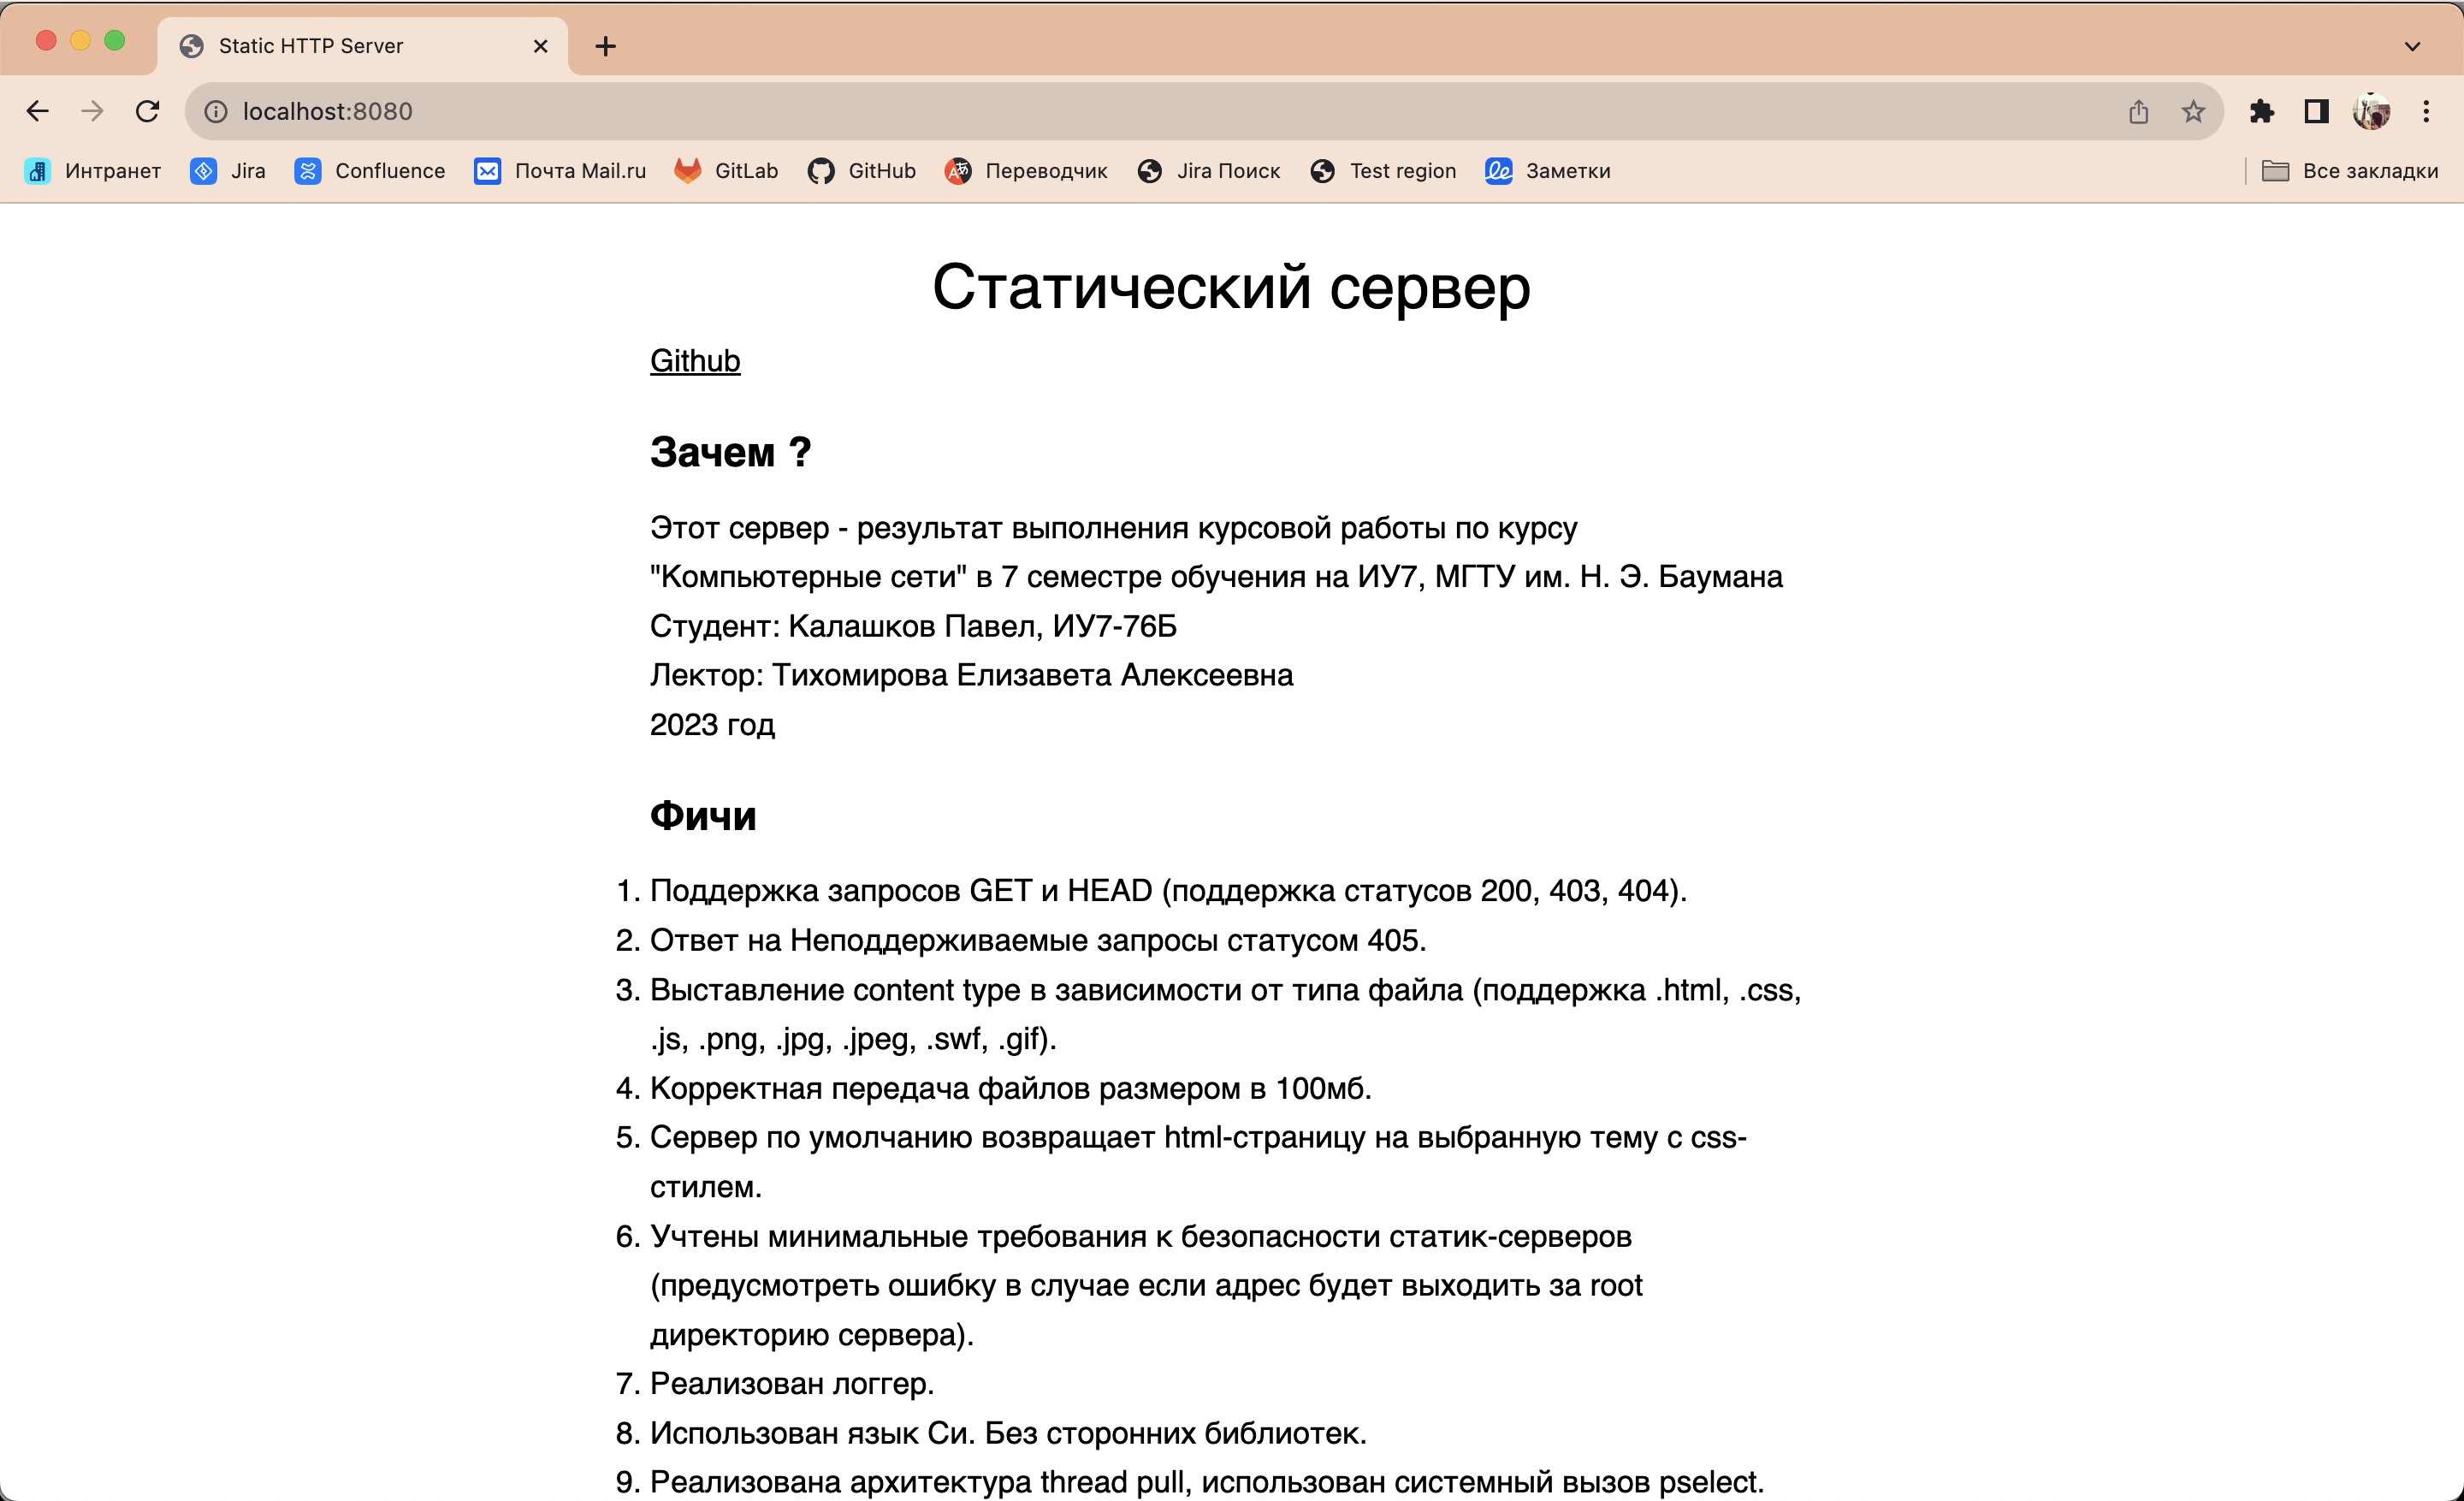
\includegraphics[width=170mm]{img/example.png}
	\caption{Базовая страница}
	\label{fig:example}
\end{figure}

\subsection{Нагрузочное тестирование}

Нагрузочное тестирование было осуществлено при помощи Apache \linebreak Benchmarks следующим образом: замерялось время обработки от 100 до 1000 (с шагом 100) запросов при подключении 5, 50 и 100 клиентами для разработанного сервера и для NGINX. 


Технические характеристики устройства, на котором выполнялось тестирование:

\begin{itemize}[label=---]
	\item Операционная система: macOS Ventura 13.2.1 (22D68) \cite{macos};
	\item Память: 16 Гб с тактовой частотой 2133 МГц LPDDR3 \cite{memory};
	\item Процессор: Intel Core™ i7-8559U \cite{intel} с тактовой частотой  2.70 ГГц;
	\item Видеокарта: Intel Iris Plus Graphics 655 \cite{graphics} c объёмом памяти 1536 Мб.
\end{itemize}

Тестирование проводилось на ноутбуке, включенном в сеть электропитания. Во время тестирования ноутбук был нагружен только системой тестирования (работающим приложением) и системным окружением операционной системы

Результаты тестирования для 5, 50 и 100 клиентов приведены на рисунках \ref{fig:test-5}, \ref{fig:test-50} и \ref{fig:test-100} соответственно. 

\begin{figure}[h]
	\centering
	\captionsetup{justification=centering}
	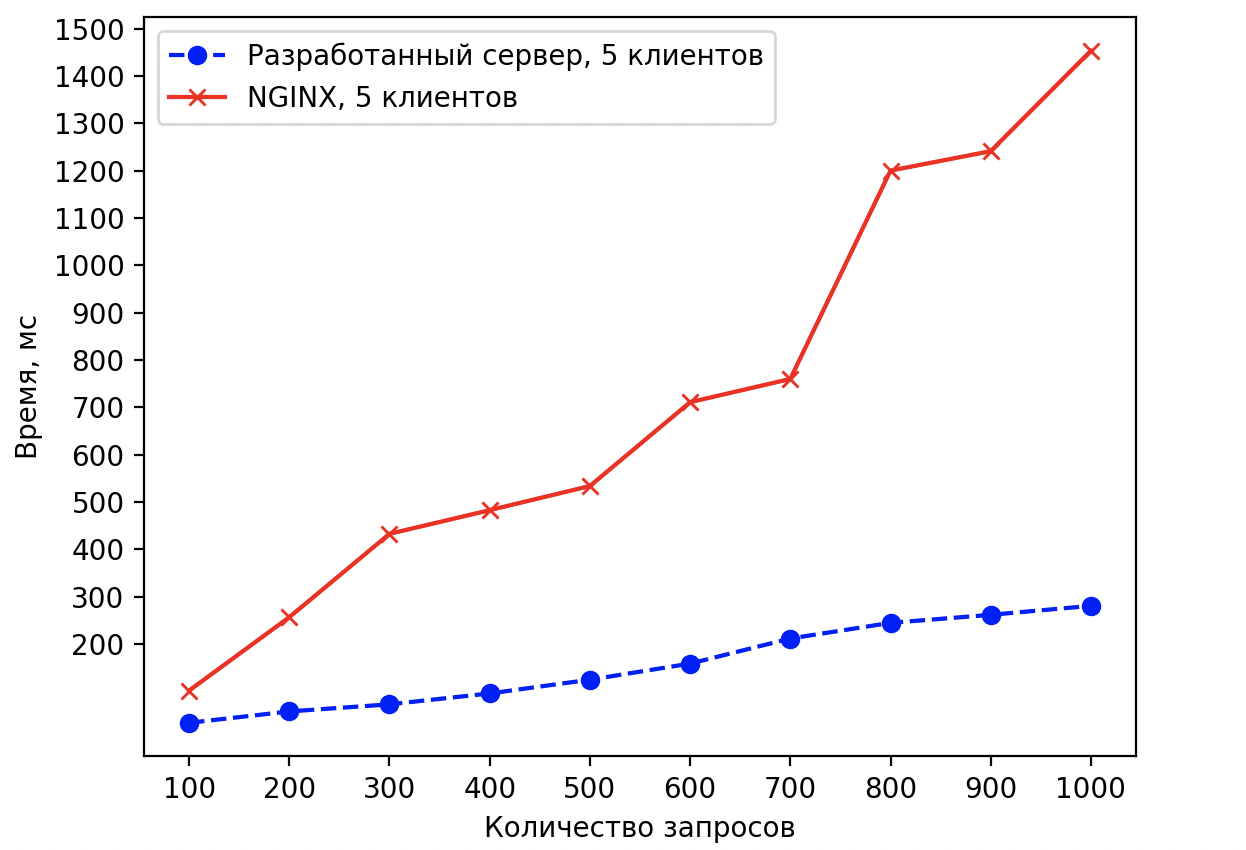
\includegraphics[width=120mm]{img/5.png}
	\caption{Результаты нагрузочного тестирования в 5 клиентов}
	\label{fig:test-5}
\end{figure}

\clearpage
\begin{figure}[h]
	\centering
	\captionsetup{justification=centering}
	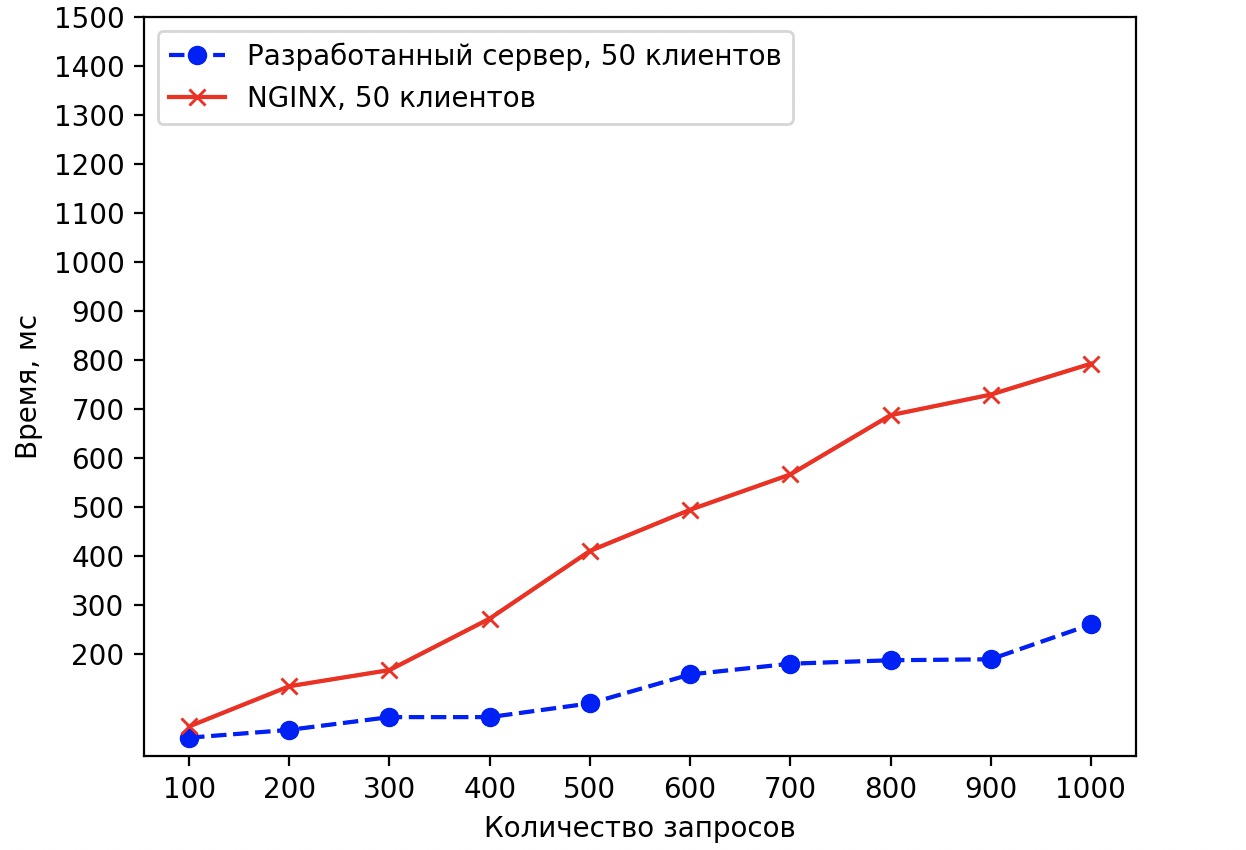
\includegraphics[width=120mm]{img/50.png}
	\caption{Результаты нагрузочного тестирования в 50 клиентов}
	\label{fig:test-50}
\end{figure}

\begin{figure}[h]
	\centering
	\captionsetup{justification=centering}
	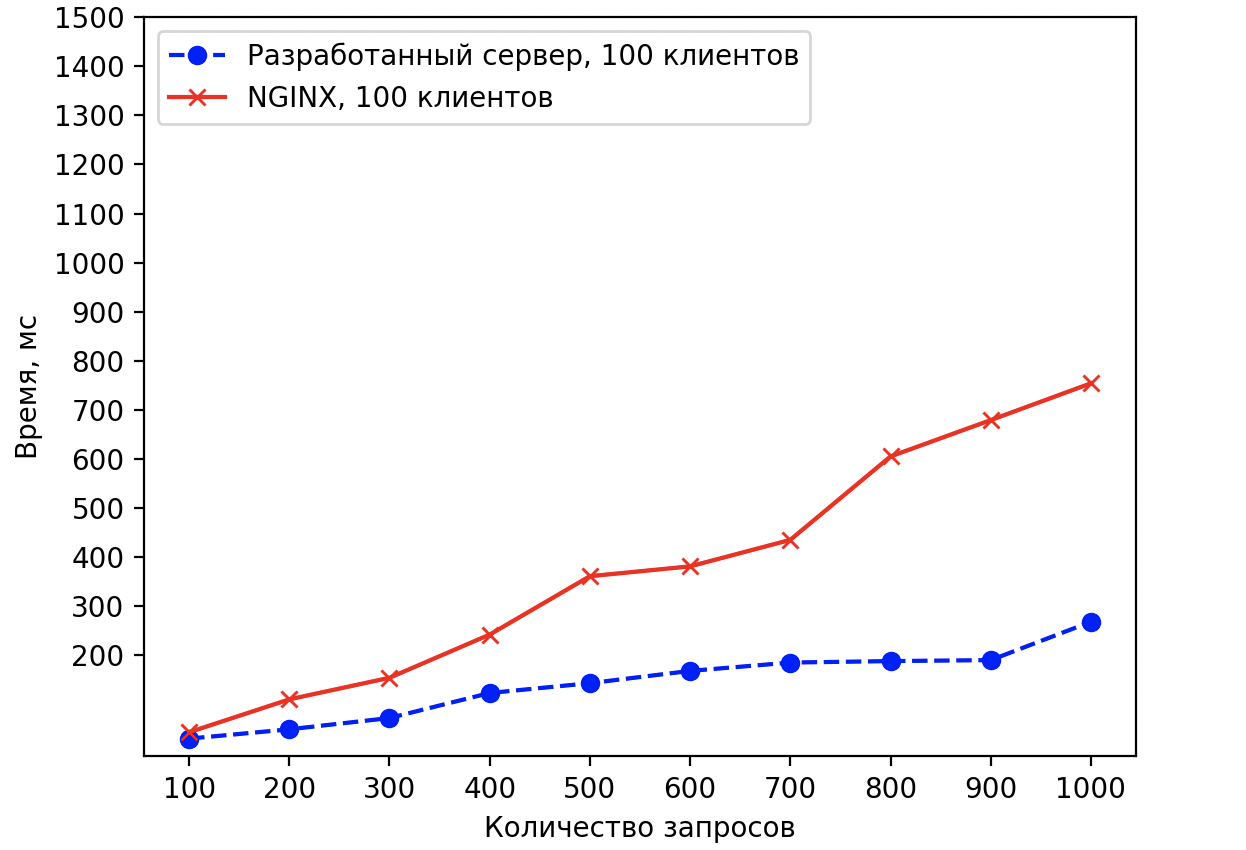
\includegraphics[width=120mm]{img/100.png}
	\caption{Результаты нагрузочного тестирования в 100 клиентов}
	\label{fig:test-100}
\end{figure}.
\clearpage

Результаты тестирования приводят к выводу, что время обработки запросов при раздаче статической информации разработанной программой меньше, чем при использовании NGINX. Чем меньше количество подсоединённых клиентов, тем больше разница во времени: так, при 1000 запросах и 5 клиентах разработанный сервер даёт разницу в 7 раз, в то время как при 50 клиентах этоо соотноошение сокращается до 3 раз. Это объясняется тем, что при замере времени обработки количество запросов оставалось одним и тем же (от 100 до 1000 с шагом 100), то есть суммарное число запросов, приходящееся на одного клиента, уменьшалось с увеличением числа клиентов.

\subsection*{Вывод}
В данном разделе были приведены примеры работы разработанной программы и проведено сравнение результатв нагрузочного тестирования, проведённого при помощи Apache Benchmarks с NGINX.

Исходя из полученных данных, при небольшом (до 100) количестве клиентов разработанная программа показывает меньшее среднее время обработки запросов, чем NGINX, при этом чем меньше клиентов подсоединено к серверу, тем больше эта разница (до 7 раз при 5 клиентах).




